\chapter*{Dodatak: Prikaz aktivnosti grupe}
		\addcontentsline{toc}{chapter}{Dodatak: Prikaz aktivnosti grupe}
		
		\section*{Dnevnik sastajanja}
		
		\textbf{\textit{Kontinuirano osvježavanje}}\\
		
		 %\textit{U ovom dijelu potrebno je redovito osvježavati dnevnik sastajanja prema predlošku.}
		
		\begin{packed_enum}
			\item  sastanak
			
			\item[] \begin{packed_item}
				\item Datum: 18. listopada 2023.
				\item Prisustvovali: Mia Krstičević, Filip Smolić, Toni Vanjak, Fran Kufrin, Dominik Šarić, Vito Tomas, Lucija Renić
				\item Teme sastanka:
				\begin{packed_item}
					\item  općenito o zadatku
					\item  alati i tehnologije
				\end{packed_item}
			\end{packed_item}
			
			\item  sastanak
			\item[] \begin{packed_item}
				\item Datum: 23. listopada 2023.
				\item Prisustvovali: Mia Krstičević, Filip Smolić, Toni Vanjak, Fran Kufrin, Dominik Šarić, Vito Tomas, Lucija Renić
				\item Teme sastanka:
				\begin{packed_item}
					\item  funkcionalnosti
					\item  zahtjevi
					\item  alati i tehnologije
				\end{packed_item}
			\end{packed_item}
			
			\item  sastanak
			\item[] \begin{packed_item}
				\item Datum: 2. studenoga 2023.
				\item Prisustvovali: Mia Krstičević, Filip Smolić, Toni Vanjak, Fran Kufrin, Dominik Šarić, Vito Tomas, Lucija Renić
				\item Teme sastanka:
				\begin{packed_item}
					\item  alati i tehnologije
					\item baza podataka
				\end{packed_item}
			\end{packed_item}
			
			\item  sastanak
			\item[] \begin{packed_item}
				\item Datum: 9. studenoga 2023.
				\item Prisustvovali: Mia Krstičević, Filip Smolić, Toni Vanjak, Fran Kufrin, Dominik Šarić, Vito Tomas, Lucija Renić
				\item Teme sastanka:
				\begin{packed_item}
					\item dosadašnji napredak
					\item arhitektura
				\end{packed_item}
			\end{packed_item}
			
			\item  sastanak
			\item[] \begin{packed_item}
				\item Datum: 14. studenoga 2023.
				\item Prisustvovali: Mia Krstičević, Filip Smolić, Toni Vanjak, Fran Kufrin, Dominik Šarić, Vito Tomas, Lucija Renić
				\item Teme sastanka:
				\begin{packed_item}
					\item dosadašnji napredak
					\item dijagram razreda
				\end{packed_item}
			\end{packed_item}
			
			\item  sastanak
			\item[] \begin{packed_item}
				\item Datum: 6. prosinca 2023.
				\item Prisustvovali: Mia Krstičević, Filip Smolić, Toni Vanjak, Fran Kufrin, Dominik Šarić, Vito Tomas, Lucija Renić
				\item Teme sastanka:
				\begin{packed_item}
					\item preraspodjela posla
				\end{packed_item}
			\end{packed_item}
			
			\item  sastanak
			\item[] \begin{packed_item}
				\item Datum: 13. prosinca 2023.
				\item Prisustvovali: Mia Krstičević, Filip Smolić, Toni Vanjak, Fran Kufrin, Dominik Šarić, Vito Tomas, Lucija Renić
				\item Teme sastanka:
				\begin{packed_item}
					\item dosadašnji napredak
					\item dijagram stanja
				\end{packed_item}
			\end{packed_item}
			
			\item  sastanak
			\item[] \begin{packed_item}
				\item Datum: 10. siječnja 2024.
				\item Prisustvovali: Mia Krstičević, Filip Smolić, Toni Vanjak, Fran Kufrin, Dominik Šarić, Vito Tomas, Lucija Renić
				\item Teme sastanka:
				\begin{packed_item}
					\item dosadašnji napredak
					\item dijagram razreda
				\end{packed_item}
			\end{packed_item}
			
			\item  sastanak
			\item[] \begin{packed_item}
				\item Datum: 16. siječnja 2024.
				\item Prisustvovali: Mia Krstičević, Filip Smolić, Toni Vanjak, Fran Kufrin, Dominik Šarić, Vito Tomas, Lucija Renić
				\item Teme sastanka:
				\begin{packed_item}
					\item dovršavanje implementacije
					\item ispitivanje programskog rješenja
				\end{packed_item}
			\end{packed_item}
			
			%
			
		\end{packed_enum}
		
		\eject
		\section*{Tablica aktivnosti}
		
			%\textbf{\textit{Kontinuirano osvježavanje}}\\
			
			 %\textit{Napomena: Doprinose u aktivnostima treba navesti u satima po članovima grupe po aktivnosti.}

			\begin{longtblr}[
					label=none,
				]{
					vlines,hlines,
					width = \textwidth,
					colspec={X[7, l]X[1, c]X[1, c]X[1, c]X[1, c]X[1, c]X[1, c]X[1, c]}, 
					vline{1} = {1}{text=\clap{}},
					hline{1} = {1}{text=\clap{}},
					rowhead = 1,
				} 
			
				\SetCell[c=1]{c}{} & \SetCell[c=1]{c}{\rotatebox{90}{\textbf{Mia Krstičević}}} & \SetCell[c=1]{c}{\rotatebox{90}{\textbf{Filip Smolić }}} &	\SetCell[c=1]{c}{\rotatebox{90}{\textbf{Toni Vanjak }}} & \SetCell[c=1]{c}{\rotatebox{90}{\textbf{Fran Kufrin }}} &	\SetCell[c=1]{c}{\rotatebox{90}{\textbf{Dominik Šarić }}} & \SetCell[c=1]{c}{\rotatebox{90}{\textbf{Vito Tomas }}} &	\SetCell[c=1]{c}{\rotatebox{90}{\textbf{Lucija Renić }}} \\  
				Upravljanje projektom 		&40  &  &  &  &  &  & \\ 
				Opis projektnog zadatka 	&  &  &  &  &  &  &8 \\ 
				
				Funkcionalni zahtjevi       &  &  &  &  &  &  &4  \\ 
				Opis pojedinih obrazaca 	&  &  &  &  &  &  &12  \\ 
				Dijagram obrazaca 			&  &  &5  &  &  &  &3  \\ 
				Sekvencijski dijagrami 		&  &  &7  &  &  &  &1  \\ 
				Opis ostalih zahtjeva 		&  &  &  &  &  &  &3  \\ 
				Arhitektura i dizajn sustava	 &  &  &6  &  &  &  &5  \\ 
				Baza podataka				&10  &  &  &  &  &  &   \\ 
				Dijagram razreda 			&  &  &6  &  &  &  &1   \\ 
				Dijagram stanja				&  &  &1  &  &  &  &3  \\ 
				Dijagram aktivnosti 		&  &  &1  &  &  &  &3  \\ 
				Dijagram komponenti			&  &  &3  &  &  &  &1  \\ 
				Korištene tehnologije i alati 		&  &  &  &  &  &  &3  \\ 
				Ispitivanje programskog rješenja 	&18  &  &  &  &  &  &15  \\ 
				Dijagram razmještaja			&  &  &3  &  &  &  &1  \\ 
				Upute za puštanje u pogon 		&  &  &  &2  &  &  &1  \\  
				Dnevnik sastajanja 			&  &  &  &  &  &  &3  \\ 
				Zaključak i budući rad 		&  &  &  &  &  &  &3  \\  
				Popis literature 			&  &  &  &  &  &  &1  \\  
				&  &  &  &  &  &  &  \\ \hline 
				\textit{Dodatne stavke kako ste podijelili izradu aplikacije} 			&  &  &  &  &  &  &  \\ 
				\textit{front end} 				&2  &170  &  &140  &  &  &  \\  
				\textit{izrada baze podataka} 		 			&63  &  &  &  &  &  & \\  
				\textit{spajanje s bazom podataka} 							&  &  &  &  &27  &30  &  \\ 
				\textit{back end} 							&65  &  &  &  &138  &150  &  \\  
				 							&  &  &  &  &  &  &\\ 
			\end{longtblr}
					
					
		\eject
		\section*{Dijagrami pregleda promjena}
		
		%\textbf{\textit{dio 2. revizije}}\\
		
		%\textit{Prenijeti dijagram pregleda promjena nad datotekama projekta. Potrebno je na kraju projekta generirane grafove s gitlaba prenijeti u ovo poglavlje dokumentacije. Dijagrami za vlastiti projekt se mogu preuzeti s gitlab.com stranice, u izborniku Repository, pritiskom na stavku Contributors.}
		
		\begin{figure}[H]
			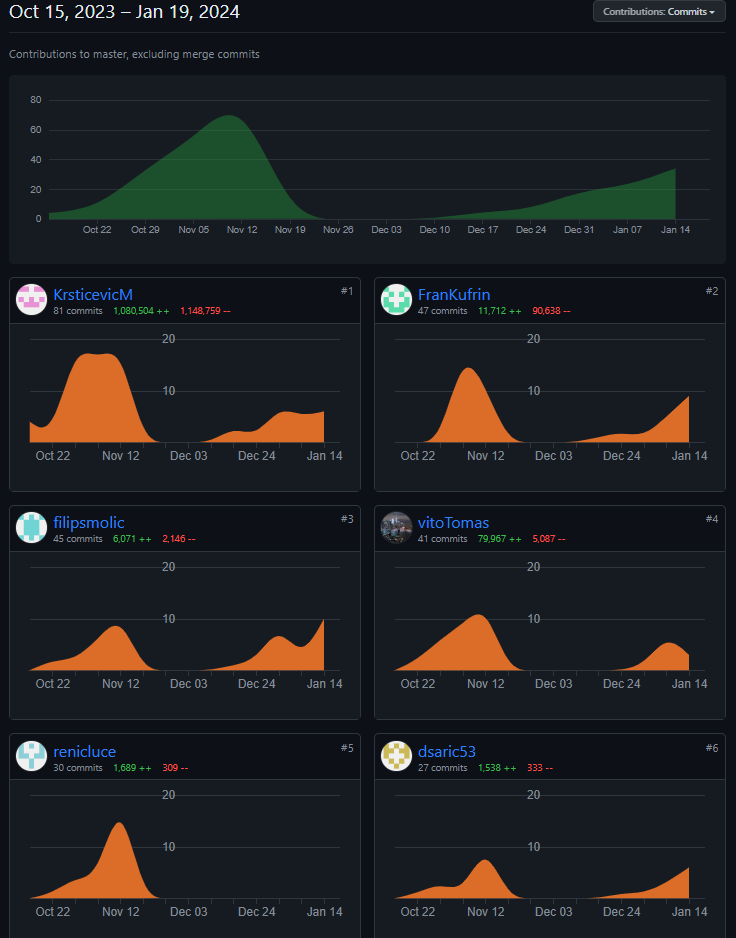
\includegraphics[width=\textwidth]{dijagramaktivnostinarepo.PNG}
			\centering
			\caption{Prikaz aktivnosti na repozitoriju}
			\label{fig:aktivnost}
		\end{figure}
	